\documentclass{article}%
\usepackage[T1]{fontenc}%
\usepackage[utf8]{inputenc}%
\usepackage{lmodern}%
\usepackage{textcomp}%
\usepackage{lastpage}%
\usepackage{authblk}%
\usepackage{graphicx}%
%
\title{Preventive effect of caffeine and curcumin on hepato\_ carcinogenesis in diethylnitrosamine\_induced rats}%
\author{Jorge Walker}%
\affil{National Creative Research Initiatives Center for Nuclear Receptor Signals, Hormone Research Center, School of Biological Sciences and Technology, Chonnam National University, Gwangju, Republic of Korea}%
\date{01{-}01{-}2011}%
%
\begin{document}%
\normalsize%
\maketitle%
\section{Abstract}%
\label{sec:Abstract}%
A new safety indication has been added to the United States Preventive Services Task Forces existing updated recommendations for sodium taurocholate as an adjunct therapy to medications for severe acute adult acute treatment of acute myocardial infarction (AMI). The S{-}PA initiative marks the first national, multi{-}centre national network of designated laboratories that provide expertise in the understanding and treatment of the incidence and causes of severe acute adult acute treatment of acute myocardial infarction (AMI). S{-}PA is a collaboration of the National Heart, Lung, and Blood Institute (NHLBI), The World Health Organization (WHO), the National Institutes of Health (NIH), and the American Academy of Clinical Oncology (AACON).\newline%
S{-}PA is recommended by the USPSTF for severely acute adult acute treatment of AMI. The Impact Ited Implementation Report (ICA) on S{-}PA was published today in the Journal of Clinical Investigation (JCI). The USPSTF is a national, independent, and interagency group of medical experts in the fields of cardiovascular disease, cancer, pediatrics, asthma, diabetes, and longevity that advises the U.S. Food and Drug Administration (FDA) about specific medical products, including dietary supplements, medical devices, and tobacco products. Under S{-}PA, the public is encouraged to view one of the JCI Assemble web sites dedicated to the topic: http://www.pssinvestigations.org/IDID989580/sbp1357 to learn more about this information.\newline%
The USPSTF uses ICA findings to inform clinical guidelines, decisions, and evaluation of new evidence for the development of a broad range of prevention therapies to reduce and eliminate AMI. Specifically, the ICA recognizes that a number of problems have arisen and that progress has been made with respect to drugs for AMI. Additional ICAs on S{-}PA are being developed in concert with the NHA.

%
\subsection{Image Analysis}%
\label{subsec:ImageAnalysis}%


\begin{figure}[h!]%
\centering%
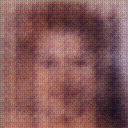
\includegraphics[width=150px]{500_fake_images/samples_5_250.png}%
\caption{A Close Up Of A Mirror On A Wall}%
\end{figure}

%
\end{document}